% ****** Start of file apssamp.tex ******
%
%   This file is part of the APS files in the REVTeX 4.1 distribution.
%   Version 4.1r of REVTeX, August 2010
%
%   Copyright (c) 2009, 2010 The American Physical Society.
%
%   See the REVTeX 4 README file for restrictions and more information.
%
% TeX'ing this file requires that you have AMS-LaTeX 2.0 installed
% as well as the rest of the prerequisites for REVTeX 4.1
%
% See the REVTeX 4 README file
% It also requires running BibTeX. The commands are as follows:
%
%  1)  latex apssamp.tex
%  2)  bibtex apssamp
%  3)  latex apssamp.tex
%  4)  latex apssamp.tex
%
\documentclass[%
 reprint,
%superscriptaddress,
%groupedaddress,
%unsortedaddress,
%runinaddress,
%frontmatterverbose,
%preprint,
%showpacs,preprintnumbers,
%nofootinbib,
%nobibnotes,
%bibnotes,
 amsmath,amssymb,
 aps,
pra,
%prb,
%rmp,
%prstab,
%prstper,
%floatfix,
]{revtex4-1}

\usepackage{graphicx}% Include figure files
\usepackage{dcolumn}% Align table columns on decimal point
\usepackage{bm}% bold math
\usepackage{enumitem}
% Stuff for Mogens' nice figure
\usepackage{braket}
\usepackage{tikz}


% Stuff for showing the algorithms
\usepackage{algorithm}
\usepackage[noend]{algpseudocode}

\newcommand{\dif}[2]{\frac{\text{d} #1}{\text{d} #2}}
\newcommand{\diff}[2]{\frac{\partial #1}{\partial #2}}
\DeclareMathOperator*{\argmin}{arg\,min}

\newcommand{\procspie}{Proceedings of the SPIE}
%\usepackage{hyperref}% add hypertext capabilities
%\usepackage[mathlines]{lineno}% Enable numbering of text and display math
%\linenumbers\relax % Commence numbering lines

%\usepackage[showframe,%Uncomment any one of the following lines to test
%%scale=0.7, marginratio={1:1, 2:3}, ignoreall,% default settings
%%text={7in,10in},centering,
%%margin=1.5in,
%%total={6.5in,8.75in}, top=1.2in, left=0.9in, includefoot,
%%height=10in,a5paper,hmargin={3cm,0.8in},
%]{geometry}

\begin{document}

%\preprint{APS/123-QED}

\title{Gradient-Based Optimal Control of Quantum Many-body Systems in Optical Lattices}% Force line breaks with \\

\author{J. J. W. H. S\o rensen}
\author{F. S. M\o ller}
\author{J. F. Sherson}
\affiliation{Aarhus University}
\email{sherson@phys.au.dk}
\date{\today}% It is always \today, today,
             %  but any date may be explicitly specified

\begin{abstract}
Abstract ...


\end{abstract}

\maketitle

\section{Introduction}

\section{Control Derivatives}


A common choice of algorithm for performing optimal control with gradients is GRAPE, where the control is discretized in steps of $\Delta t$. While the gradient of the cost functional in the original algorithm was derived to $O(\Delta t ^2)$ precision, a series of higher order corrections were added in CITE. The resulting gradient reads
\begin{equation}
	\frac{\partial J}{\partial u_n (t_j)}  = - \Re \Braket{\chi (t_j) | i  \frac{\partial \hat{\mathcal{U}}_{t_j}}{\partial u_n (t_j)} | \psi (t_{j-1})} \; ,
\end{equation} 
where the derivative of the propagator with respect to the control is given by
\begin{equation}
	\frac{\partial \hat{\mathcal{U}}_{j}}{\partial u_n (t_j)} = e^{-i \hat{H} (u_n (t_j)) \Delta t}  \sum_{k = 0}^{\infty }  \frac{i^{k} \Delta t^{k+1}}{(k+1)!} \left[ \hat{H} (u_n (t_j)) , \frac{\partial \hat{H} (u_n (t_j))}{\partial u_n (t_j)}  \right]_k \; . 
\end{equation}
The first order term of the recursive commutator, $\frac{\partial \hat{H}}{\partial u_n (t_j)}$, produces the gradient of the original GRAPE algorithm.\\
Since the control function, and thereby the Hamiltonian, is repeatedly modified during the optimization procedure, the propagator most be re-calculated multiple times. This is costly, as exponentiating the Hamiltonian is a non-trivial operation. Non-updated parts of the propagator can be re-used, by expanding the propagator through the Suzuki-Trotter expansion 
\begin{equation}
		e ^{( \hat{H}_n + \hat{H}_0  ) \delta } = e^{  \hat{H}_n \delta /2  } e^{ \hat{H}_0 \delta } e^{ \hat{H}_n \delta /2 } + O(\delta^3) \; . \label{eq:SuzukiTrotter}
\end{equation}
Calculating the propagator can be done very efficiently, if the controllable part of the Hamiltonian is diagonal. Thereby, the repeated exponentiation is trivial, while constant, non-diagonal parts of the Hamiltonian can be exponentiated separately at the start of the optimization.\\
Consider the Suzuki-Trotter expansion of eq. \eqref{eq:SuzukiTrotter}, where the Hamiltonian $\hat{H}_n$ is diagonal. Additional accuracy can be achieved by evaluating $\hat{H}_n$ using the midpoint rule, i.e. when evolving the state from $t_{j-1} \to t_j$ propagate first using $\hat{H}_n (u (t_{j-1}))$ followed by $\hat{H}_n (u (t_{j}))$ at the end of the expansion. Utilizing the midpoint rule along with the Suzuki-Trotter expansion also has profound impact on the  gradient, as all higher-order contributions vanish.
Expressing the Suzuki-Trotter expanded propagator as
\begin{equation}
	\hat{\mathcal{U}}_{j}^{\mathrm{ST}} = e^{ -i  \hat{H}_n (u (t_j)) \Delta t /2 } e^{ -i \hat{H}_0 \Delta t } e^{ -i  \hat{H}_n (u (t_{j-1}))  \Delta t /2 }  \equiv \hat{\mathcal{U}}_{j}^{(n)} \hat{\mathcal{U}}_{j}^{(0)} \hat{\mathcal{U}}_{j-1}^{(n)} \; , 
\end{equation}
makes it clear that both $\mathcal{U}_{j}^{\mathrm{ST}}$ and $\mathcal{U}_{j+1}^{\mathrm{ST}}$ contribute to $\frac{\partial J}{\partial u_n (t_j)}$.
Further examining the derivative of the first propagator reveals
\begin{align}
	\frac{\partial \hat{\mathcal{U}}_{j}^{\mathrm{ST}}}{\partial U (t_j)} &=  \frac{\partial \hat{\mathcal{U}}_{j}^{(n)}}{\partial U (t_j)} \hat{\mathcal{U}}_{j}^{(0)} \hat{\mathcal{U}}_{j-1}^{(n)} \nonumber \\
	&=  e^{ -i U (t_j) \hat{H}_n  \Delta t /2 }  \sum_{k = 0}^{\infty }  \frac{i^k \Delta t^{k+1}}{(k+1)!} \left[ \hat{H}_n (u_n (t_j))  ,  \frac{\partial \hat{H}_n (u_n (t_j))}{\partial u_n (t_j)} \right]_k \hat{\mathcal{U}}_{j}^{J} \hat{\mathcal{U}}_{j-1}^{U} \nonumber \\
	&= \left(  \hat{H}_n (u_n (t_j)) \Delta t /2 \right) \hat{\mathcal{U}}_{j}^{\mathrm{ST}} \; . \label{eq:STpropderiv1}
\end{align}
Since $\hat{H}_n$ is diagonal, the recursive commutator is vanishing for $k > 0$, which causes all higher-order contributions to the derivative of the propagator to drop out.\\
Likewise, the derivative of the second propagator is
\begin{equation}
	\frac{\partial \hat{\mathcal{U}}_{j+1}^{\mathrm{ST}}}{\partial u_n (j)} =  \hat{\mathcal{U}}_{j+1}^{\mathrm{ST}} \left(  \hat{H}_n (u_n (t_j)) \Delta t /2 \right) \; . \label{eq:STpropderiv2}
\end{equation}
Inserting the derivatives of eq. \eqref{eq:STpropderiv1} and \eqref{eq:STpropderiv2} into the derivative of the cost (eq. \eqref{eq:STcostderiv}) yields
\begin{align}
	\frac{\partial J}{\partial u_n (t_j)} &= - \Re \Braket{\chi (t_j) | i  \left(  \hat{H}_n (u_n (t_j)) \Delta t /2 \right) \hat{\mathcal{U}}_{j}^{\mathrm{ST}} | \psi (t_{j-1})} - \Re \Braket{\chi (t_{j+1}) | i \hat{\mathcal{U}}_{j+1}^{\mathrm{ST}} \left(  \hat{H}_n (u_n (t_j)) \Delta t /2 \right) | \psi (t_{j})} \nonumber \\
	&= - \Re \Braket{\chi (t_j) | i \hat{H}_n (u_n (t_j)) \Delta t | \psi (t_{j})} \; . \label{eq:STcostgrad}
\end{align}  
Thus, the combination of the Suzuki-Trotter expansion and a diagonal control Hamiltonian eliminates all higher order contributions to the gradient. Thereby, the gradient of the cost is exact up to the order of the expansion.

  

\section{Results}


\begin{figure}[h!]
    \centering
    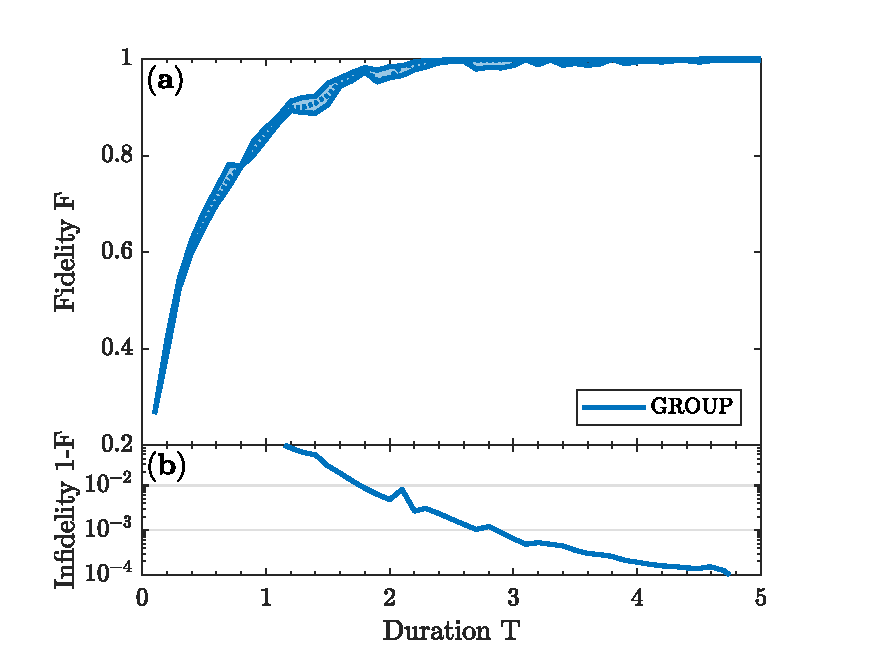
\includegraphics[width=0.45\textwidth]{Figures/FidelityDuration.pdf}
    \caption{\textit{Final fidelity obtained for optimal control at various durations. \textbf{(a)} the dotted line marks the median fidelity achieved, while the shaded area displays the $25\%$- and $75\%$-quartiles of the solutions. \textbf{(b)} the lowest infidelity achieved for each duration. }}
    \label{fig:FidelityDuration}
\end{figure}

\begin{figure}[h!]
    \centering
    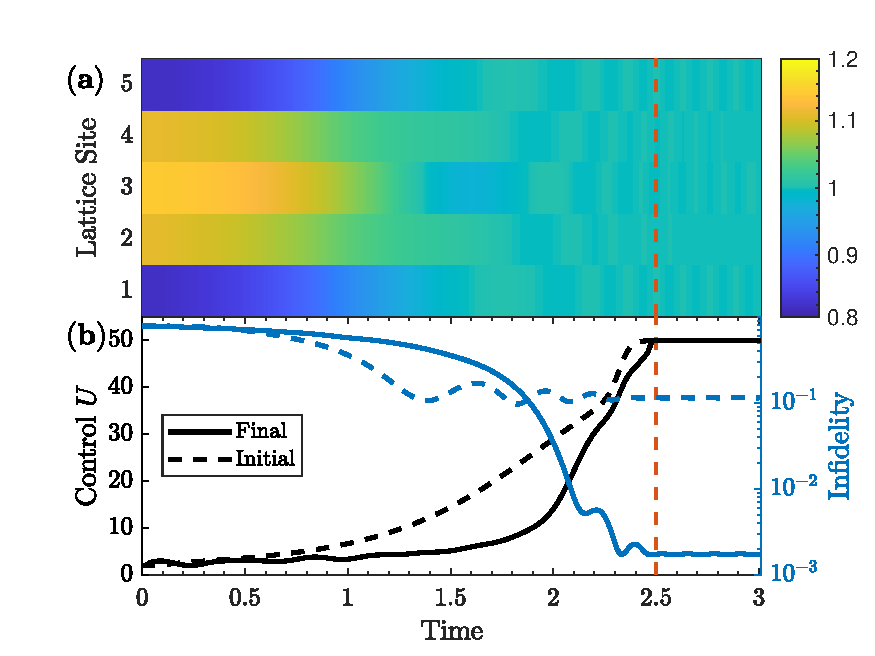
\includegraphics[width=0.45\textwidth]{Figures/OptRamp.pdf}
    \caption{\textit{Solution with highest fidelity achieved for duration $T = 2.5$. The dashed, red line marks the end of the duration, from which the system is further evolved using the final control value. \textbf{(a)} logarithmically scaled expectation value of the number operator, $\braket{\hat{n}_i}$, for each site, as the system is evolved according to the optimized ramp. \textbf{(b)} the initial and optimized ramp sequences along with the corresponding evolution of fidelities.}}
    \label{fig:OptRamp}
\end{figure}

\begin{figure}[h!]
    \centering
    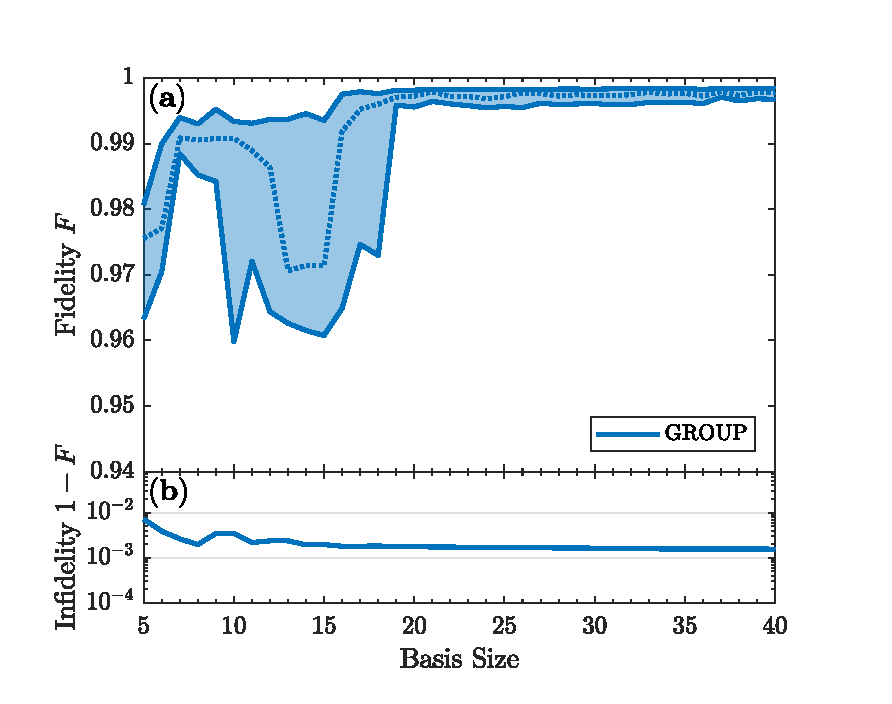
\includegraphics[width=0.45\textwidth]{Figures/FidelityBasisSize.pdf}
    \caption{\textit{Final fidelity obtained for optimal control at various optimization space dimensions for duration $T = 2.5$. \textbf{(a)} the dotted line marks the median fidelity achieved, while the shaded area displays the $25\%$- and $75\%$-quartiles of the solutions. \textbf{(b)} the lowest infidelities achieved for each basis size.}}
    \label{fig:FidelityBasisSize}
\end{figure}

\begin{figure}[h!]
    \centering
    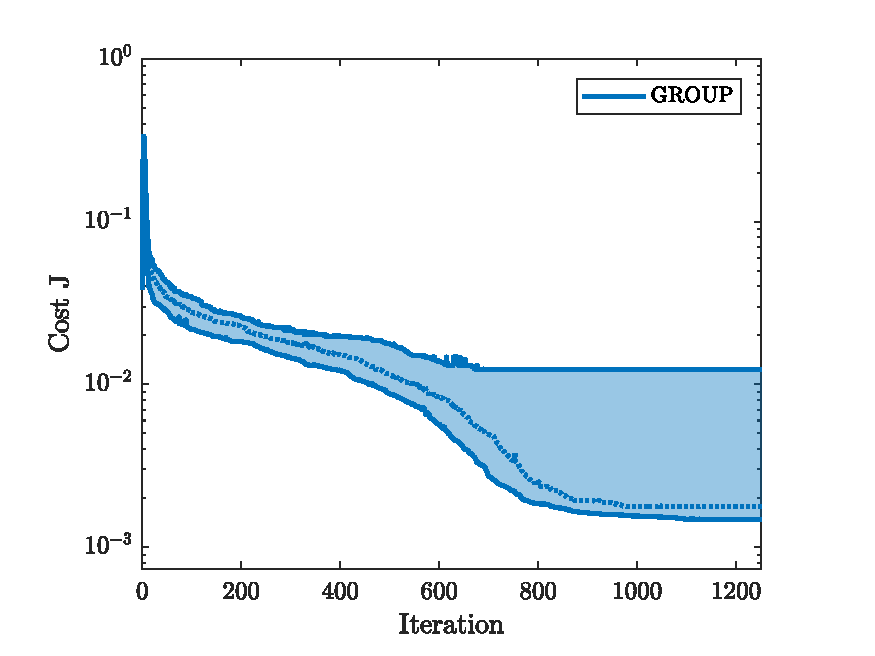
\includegraphics[width=0.45\textwidth]{Figures/CostProgress.pdf}
    \caption{\textit{The value of the cost function at a given number of time evolutions. The dotted line marks the median and the shaded area indicates the $25\%$- and $75\%$-quartiles found from X different random initial controls.}}
    \label{fig:FidelityBasisSize5}
\end{figure}


%\bibliographystyle{apsrev4-1}
%\bibliography{references}

\end{document}
%
% ****** End of file apssamp.tex ******
